\documentclass{ctexbook}

%%%%%%%%%%%%%%%%%%%%%%%%%%%%%%%%%%%%
\usepackage[backend=bibtex,style=gb7714-2015]{biblatex}
\addbibresource[location=local]{reference.bib} % 参考文献,不要删除
\DeclareSortingTemplate{c}{\sort{\citeorder}}
\ExecuteBibliographyOptions{sorting=c}

\usepackage{makeidx} % 调用 makeidx 宏包,用来处理索引
\makeindex % 开启索引的收集
\usepackage[nottoc]{tocbibind}  % 使得目录中显示"索引"
\usepackage[totoc,columns=2]{idxlayout}

% hyperref with xcolor
\usepackage[dvipsnames]{xcolor}
\usepackage{hyperref}
\hypersetup{
    colorlinks=true,
    linkcolor=blue!50!red,
    urlcolor=green!70!black
}


% 代码高亮设置%
\usepackage{listings}
\lstset{ %
  numbers=left,
  numberstyle=\tiny,
  frame=shadowbox,
  backgroundcolor=\color{white},   % choose the background color
  basicstyle=\ttfamily,        % size of fonts used for the code
  breaklines=true,                 % automatic line breaking only at whitespace
  captionpos=b,                    % sets the caption-position to bottom
  commentstyle=\color{Gray},    % comment style
  keywordstyle=\color{teal},       % keyword style
  stringstyle=\color{Tan},     % string literal style
  showstringspaces=false,
}


\usepackage{graphicx}

% 公式高亮
%%% standard math packages for equations:
\usepackage{amsmath}
\usepackage{amssymb}
\usepackage{mathtools}
\usepackage{cleveref}
\usepackage{annotate-equations}


%%%%%%%%%%%%%%%%%%%%%%%%%%%%%%%%%%%%


\begin{document}

%%%%%%%%%%%%%%%%%%%%%%%%%%%%%%%%%%%%
% Title page, table of contents, etc.
\frontmatter
\begin{titlepage}
    \begin{center}
        \vspace*{1cm}
 
        \textbf{\zihao{1}一个不太复杂的中文书籍\LaTeX 模板}
 
        \vspace{0.5cm}
        \zihao{-2} 基于 ctexbook 的极简模板
             
        \vspace{0.5cm}

        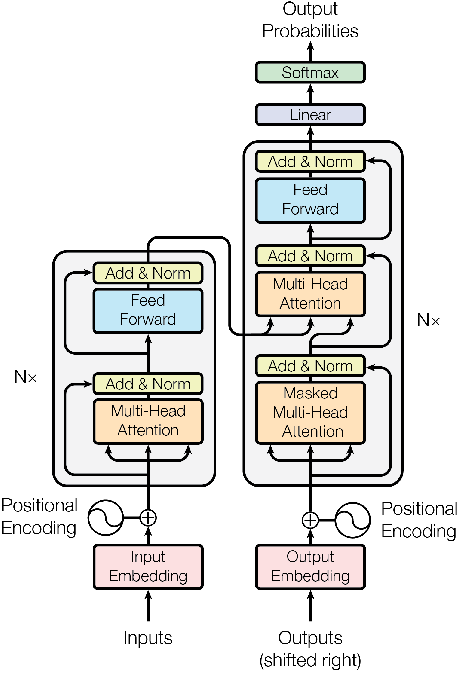
\includegraphics[width=0.6\textwidth]{./figures/transformer.pdf}

        \vfill

        \vspace{0.5cm}
        \textbf{Mathew Shen} \\
        \today \hspace{1cm} V0.0.1

    \end{center}
 \end{titlepage}


% 增加目录
\tableofcontents
% 目录设置:深度
\setcounter{tocdepth}{2}

% 前言
\chapter{前言}
旨在建立一个简单通用又不失美观的\LaTeX 中文书籍模板。

%%%%%%%%%%%%%%%%%%%%%%%%%%%%%%%%%%%%


%%%%%%%%%%%%%%%%%%%%%%%%%%%%%%%%%%%%
% Main body of the document
\mainmatter
\chapter{环境配置}

\LaTeX 开发环境配置。

\section{\LaTeX 环境安装}
\index{环境安装}

\begin{itemize}
    \item \TeX Live 安装
    \item 安装 VsCode,安装\LaTeX Workshop 插件
    \item SumatraPDF 阅读器 (可选,用于预览生成的 PDF 文件)
\end{itemize}


\section{IDE 配置}
\index{IDE}
\index{VsCode}

\LaTeX Workshop recipes 设置 latexmk:

\begin{lstlisting}
"latex-workshop.latex.tools": [
  {
    "name": "latexmk",
    "command": "latexmk",
    "args": [
      "--shell-escape",
      "-synctex=1",
      "-interaction=nonstopmode",
      "-file-line-error",
      "-xelatex",
      "%DOC%"
    ]
  },
],

  "latex-workshop.latex.recipes": [
  {
    "name": "latexmk",
    "tools": [
        "latexmk"
      ]
  },
],
\end{lstlisting}


\chapter{ctexbook 使用简介}
\label{chap:ctexbook}

中文文档类测试。你需要将所有源文件保存为 UTF-8 编码。
你可以使用 XeLaTeX、LuaLaTeX 或 upLaTeX 编译,也可以使用 (pdf)LaTeX 编译。
推荐使用 XeLaTeX 或 LuaLaTeX 编译。对高级用户,我们也推荐使用 upLaTeX 编译。



\section{代码}
\index{代码}


下面是一段 Python 代码
\footnote{综合考量\textit{lstlisting}和\textit{minted}之后还是决定选前者,牺牲了一些语言的默认样式,但总体更加常用一些,也更安全 (不用\textit{-shell-escape})。}:
\begin{lstlisting}[language=python, caption={Python 代码示例}]
def hello_world():
    print("Hello, World!")
\end{lstlisting}


\section{数学公式}
\index{数学公式}
\index{Attention}

我们可以通过公式\ref{attention_equation}来定义 Attention。
\begin{equation}\label{attention_equation}\index{transformer}
    Attention(Q, K, V) = softmax(\frac{QK^T}{\sqrt{d_k}})V
\end{equation}

这里通过\texttt{\textbackslash label}来标识公式,通过\texttt{\textbackslash ref}来引用公式。

\section{引用文献}
\index{文献}
引用一个文献\cite{siffer2017anomaly}。


\section{图片}
插入 PDF 矢量图:

\begin{figure}[htbp]
    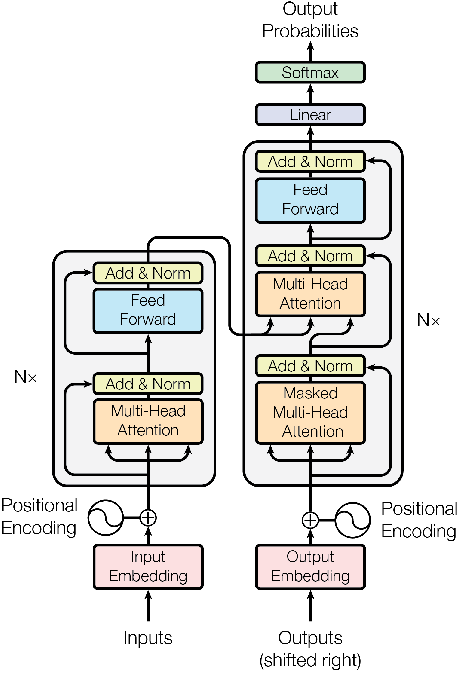
\includegraphics[width=0.6\textwidth]{./figures/transformer.pdf}
    \centering
    \caption{Transformer 架构\cite{vaswani2017attention}}
    \index{transformer}
\end{figure}

\chapter{目录与附录}
介绍如何配置目录,附录等。


\section{附录}

\subsection{参考文献}
引用一个文献\cite{siffer2017anomaly}。  % 这里带上.tex 也是可以的

%%%%%%%%%%%%%%%%%%%%%%%%%%%%%%%%%%%%



%%%%%%%%%%%%%%%%%%%%%%%%%%%%%%%%%%%%
% Appendices, bibliography, etc.
\backmatter

% 附录
\chapter{附录A}
附录A的内容。



% 参考文献
\printbibliography[title={参考文献}, heading=bibintoc]

% 索引
\printindex

%%%%%%%%%%%%%%%%%%%%%%%%%%%%%%%%%%%%

\end{document}